\documentclass[12pt,a4paper,oneside]{report}

\usepackage[utf8]{inputenc}
\usepackage{graphicx}
\usepackage{geometry}
\usepackage{hyperref}
\usepackage{titlesec}
\usepackage{etoolbox}
\usepackage{float}
\usepackage{setspace}
\usepackage{amsmath}
\usepackage{amssymb}
\usepackage{listings}
\usepackage{xcolor}
\usepackage{caption}
\usepackage{subcaption}
\usepackage{enumitem}
\usepackage{booktabs}
\usepackage{multirow}
\usepackage{tabularx}
\usepackage{tikz}
\usetikzlibrary{shapes.geometric,arrows.meta,positioning,fit,backgrounds,calc,matrix}

% -------------------------------------------------------------------
% PAGE GEOMETRY
% -------------------------------------------------------------------
\geometry{
    left=25mm,
    right=25mm,
    top=20mm,
    bottom=22mm,
    headsep=10pt
}

% -------------------------------------------------------------------
% LINE & PARAGRAPH SPACING
% -------------------------------------------------------------------
\setstretch{1.15}
\setlength{\parskip}{4pt}
\setlength{\parindent}{15pt}
\raggedbottom

% -------------------------------------------------------------------
% NEUTRALISE HARDCODED TOP SPACING IN REPORT CLASS
% -------------------------------------------------------------------
\makeatletter
\patchcmd{\@makechapterhead}{\vspace*{50\p@}}{}{}{}
\patchcmd{\@makeschapterhead}{\vspace*{50\p@}}{}{}{}
\makeatother

% -------------------------------------------------------------------
% CHAPTER / SECTION FORMATTING
% -------------------------------------------------------------------
\titleformat{\chapter}[display]
  {\normalfont\huge\bfseries}
  {\chaptertitlename\ \thechapter}
  {10pt}
  {\Huge}

\titlespacing*{\chapter}{0pt}{0pt}{18pt}
\titlespacing*{\section}{0pt}{10pt}{6pt}
\titlespacing*{\subsection}{0pt}{8pt}{4pt}

\setlength{\textfloatsep}{12pt}
\setlength{\floatsep}{10pt}
\setlength{\intextsep}{10pt}
\setlist{nosep}

% -------------------------------------------------------------------
% COLOR PALETTE & HYPERREF
% -------------------------------------------------------------------
\definecolor{brandPrimary}{RGB}{99,102,241}
\definecolor{brandDark}{RGB}{67,56,202}
\definecolor{brandSecondary}{RGB}{243,244,246}
\definecolor{brandSuccess}{RGB}{16,185,129}
\definecolor{brandDanger}{RGB}{239,68,68}
\definecolor{codeBg}{RGB}{248,250,252}

\hypersetup{
    colorlinks=true,
    linkcolor=brandDark,
    citecolor=brandPrimary,
    urlcolor=brandDark
}

% -------------------------------------------------------------------
% CODE LISTING STYLE
% -------------------------------------------------------------------
\lstset{
    basicstyle=\ttfamily\footnotesize,
    breaklines=true,
    backgroundcolor=\color{codeBg},
    frame=single,
    rulecolor=\color{gray!30},
    numbers=left,
    numberstyle=\tiny\color{gray},
    keywordstyle=\color{brandPrimary}\textbf,
    stringstyle=\color{brandSuccess!70!black},
    commentstyle=\color{gray},
    showstringspaces=false,
    captionpos=b,
    tabsize=2
}

\begin{document}

% ===================================================================
% 1. TITLE PAGE
% ===================================================================
\begin{titlepage}
    \centering
    \vspace*{1.0cm}
    
    {\Huge \textbf{MNEME: AN AI-POWERED ACTIVE RECALL AND COGNITIVE RETENTION PLATFORM}\par}
    \vspace{0.6cm}
    {\Large \textsc{End Semester Examination Capstone Technical Project}\par}
    
    \vspace{1.2cm}
    \begin{center}
        
\begin{tikzpicture}
            \draw[brandPrimary, fill=brandPrimary!10, rounded corners=12pt, line width=1.5pt] (0,0) rectangle (6,2.2);
            \node at (3,1.4) {\Large \textbf{MNEME}};
            \node at (3,0.7) {\footnotesize \textit{Intelligent Spaced Repetition and Retrieval Studio}};
        \end{tikzpicture}
    \end{center}
    
    \vspace{1.2cm}
    {\large \textbf{Submitted by:}\par}
    \vspace{0.2cm}
    {\large Aryan Tikam\par}
    {\normalsize Department of Computer Engineering / Computer Science\par}
    
    \vspace{1.5cm}
    {\large \textbf{Under the Guidance of:}\par}
    \vspace{0.2cm}
    {\normalsize Project Evaluation Committee and Department Faculty\par}
    
    \vfill
    {\normalsize Academic Term: Autumn 2026\par}
    {\normalsize Date of Submission: November 2026\par}
\end{titlepage}

% ===================================================================
% 2. INDEX / TABLE OF CONTENTS
% ===================================================================
\pagenumbering{roman}
\tableofcontents
\newpage
\listoffigures
\newpage
\listoftables
\newpage

% ===================================================================
% 3. ABSTRACT
% ===================================================================
\addcontentsline{toc}{chapter}{Abstract}
\chapter*{Abstract}

Traditional academic review practices rely heavily on passive rereading and rote highlighting. Empirical educational neuroscience demonstrates that these passive modalities produce rapid cognitive decay along the Ebbinghaus forgetting curve, with retention falling below 30 percent within forty-eight hours. Mneme is an end-to-end active recall and spaced repetition learning system engineered to transform raw educational literature into verifiable long-term semantic memory. The platform accepts unstructured multimodal lecture documents (PDF, Markdown, plain text), partitions them via semantic chunking algorithms, and embeds them into isolated tenant vector partitions in a Qdrant vector database.

The computational core leverages Groq Language Processing Units (LPU) serving the Qwen 2.5/3.8 27B-Instruct parameter model. A distributed Celery worker pool decoupled through Redis coordinates asynchronous indexing and deterministic card synthesis. To ensure structural reliability, generative outputs are governed by cyclical LangGraph state machines equipped with Pydantic schema validation barriers. In addition to spaced-repetition flashcards and multiple-choice diagnostic quizzes, Mneme introduces two novel interactive cognitive paradigms: Blurt Mode and the Socratic Feynman Tutor. Blurt Mode performs automated semantic difference evaluation between unrestrained student free-recall blurts and source text, extracting recalled concepts, pinpointing knowledge voids, and issuing a grounded retention score. The Feynman Tutor utilizes an intent router to engage learners Socratically or challenge them as Richard Feynman to explain concepts without technical jargon, graded dynamically via deterministic Flesch Reading Ease metrics. Built on a resilient stack featuring React 19, Tailwind CSS, Flask, and MongoDB Atlas, Mneme enforces absolute multi-tenant tenant isolation and live per-user cognitive mastery tracking.

\newpage
\pagenumbering{arabic}

% ===================================================================
% 4. INTRODUCTION
% ===================================================================
\chapter{Introduction}

\section{Background and Problem Statement}
In higher education and technical professions, students and practitioners encounter vast quantities of dense, highly conceptual literature. Typical studying strategies consist of passive linear reading, transcription, and manual document highlighting. Decades of cognitive psychology research show that passive review creates an illusion of competence: learners recognize terminology while being unable to reconstruct arguments or solve novel problems under examination pressure.

According to Hermann Ebbinghaus's mathematical formulation of human memory decay, newly acquired information decays exponentially if unreinforced:
\begin{equation}
    R(t) = e^{-\frac{t}{S}}
\end{equation}
where $R$ denotes memory retrievability, $t$ is elapsed time, and $S$ represents memory stability. When students rely solely on pre-exam cramming, $S$ remains low, causing learned concepts to deteriorate rapidly post-assessment. 

The two most empirically proven methodologies for flattening this decay curve are:
\begin{enumerate}
    \item \textbf{Active Recall (The Testing Effect):} Forcing the brain to retrieve concepts from memory without looking at notes strengthens synaptic pathways far more effectively than passive observation.
    \item \textbf{Spaced Repetition Systems (SRS):} Scheduling recall intervals precisely when retrievability $R$ drops toward the forgetting threshold maximizes memory stability gains per unit of study time.
\end{enumerate}

Despite their demonstrated efficacy, manual creation of high-quality active recall artifacts (atomic flashcards, diagnostic multiple-choice questions, concept comparison grids) imposes prohibitive cognitive friction. Manually authoring comprehensive flashcard decks for a 400-page engineering textbook requires dozens of hours, leading most students to abandon spaced repetition in favor of passive review.

\section{Project Objectives}
Mneme was conceived and developed to eliminate the friction of active recall artifact creation through automated, high-fidelity neural synthesis. The project encompasses the following foundational engineering objectives:
\begin{itemize}
    \item \textbf{Automated Concept Ingestion:} Ingest complex academic documents, extract structural headings and body text, and chunk content semantically to preserve mathematical and logical continuity.
    \item \textbf{Deterministic AI Generation:} Deploy cyclical state machines through LangGraph and Pydantic validation to generate pedagogically rigorous flashcards and diagnostic quizzes with guaranteed zero schema breakage.
    \item \textbf{Segregated Multi-Document Contexts:} Enable users to upload arbitrary numbers of documents into a central library and bind or detach individual documents to specific decks, establishing isolated context boundaries for synthesis.
    \item \textbf{Semantic Blurt Recall Auditing:} Implement an automated blurt evaluation pipeline that vectors student free-recall submissions, retrieves source grounding from Qdrant, and computes an objective semantic diff separating remembered concepts from critical omissions.
    \item \textbf{Socratic and Feynman Pedagogical Mentorship:} Deliver a real-time Server-Sent Events (SSE) conversational tutor capable of distinguishing user questions from student conceptual explanations, providing Socratic guidance and enforcing plain-English clarity through automated readability scoring.
    \item \textbf{Data Privacy and Multi-Tenant Isolation:} Enforce cryptographic user authentication and strict payload-level filtering across all database queries and vector searches.
\end{itemize}

\section{Cognitive Science Foundations}
Mneme synthesizes four established paradigms in cognitive science into a unified technical application:

\subsection{SuperMemo-2 and Free Spaced Repetition (FSRS)}
The core flashcard scheduling engine is modeled on spaced repetition principles where inter-repetition intervals grow exponentially:
\begin{equation}
    I(1) = 1, \quad I(2) = 6, \quad I(n) = I(n-1) \times EF
\end{equation}
where $I(n)$ is interval length in days for repetition $n$, and $EF$ is the dynamic ease factor updated according to student performance ratings.

\subsection{The Feynman Technique}
Named after Nobel laureate Richard Feynman, this technique posits that true mastery of a concept is demonstrated by the ability to explain it in simple, jargon-free language to an uninitiated audience. When learners hide behind technical jargon, they frequently mask gaps in conceptual understanding.

\subsection{The Blurt Method}
The Blurt Method involves reading a chapter, closing all materials, and writing down every remembered principle, formula, and connection onto a blank page. Performing an immediate audit against source notes highlights hidden cognitive blindspots.

\newpage

% ===================================================================
% 5. APPLICATION WORKFLOW AND SYSTEM ARCHITECTURE
% ===================================================================
\chapter{Application Workflow and System Architecture}

\section{High-Level Architectural Overview}
Mneme is engineered as a decoupled, asynchronous microservices-oriented web application. The technical stack spans five primary layers:
\begin{enumerate}
    \item \textbf{Presentation Layer (Frontend):} Built with React 19, TypeScript, TanStack Router, Tailwind CSS, and Framer Motion. Implements responsive navigation, tactile 3D swipeable flashcards, real-time SSE chat drawers, and multi-folder deck management.
    \item \textbf{Application Gateway (REST API):} Implemented in Python using Flask and Werkzeug, providing endpoints for document upload, asynchronous task tracking, authentication, CRUD deck manipulation, and SSE streaming.
    \item \textbf{Asynchronous Worker Pool:} Celery workers driven by Redis handle long-running CPU-bound tasks (PDF extraction, embedding synthesis, cyclical LangGraph LLM generation) without blocking HTTP threads.
    \item \textbf{Vector and Relational Storage Layer:} Qdrant vector database handles high-dimensional dense vector embeddings with strict tenant payload filtering. MongoDB Atlas serves as the primary document store for users, folders, decks, cards, and daily activity logs.
    \item \textbf{Inference Engine:} Groq Cloud Language Processing Units running Qwen 2.5/3.8 27B-Instruct, delivering generation speeds exceeding 140 tokens per second.
\end{enumerate}

\begin{figure}[H]
\centering
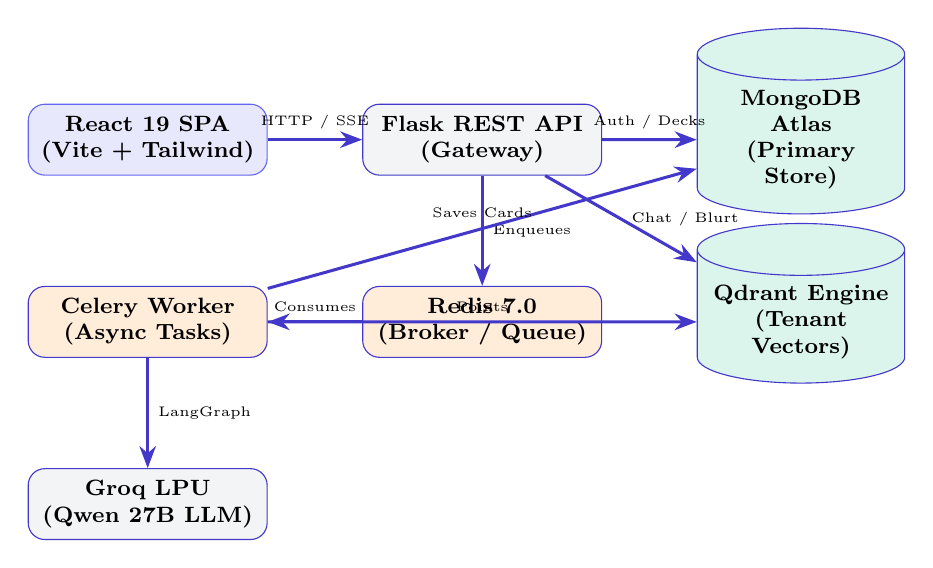
\begin{tikzpicture}[
    node distance=1.4cm and 1.2cm,
    box/.style={rectangle, draw=brandDark, fill=brandSecondary, rounded corners=6pt, text centered, minimum height=0.9cm, text width=2.8cm, font=\footnotesize\bfseries},
    clientbox/.style={rectangle, draw=brandPrimary, fill=brandPrimary!15, rounded corners=6pt, text centered, minimum height=0.9cm, text width=2.8cm, font=\footnotesize\bfseries},
    dbbox/.style={cylinder, draw=brandDark, fill=brandSuccess!15, shape border rotate=90, aspect=0.25, text centered, minimum height=1.1cm, text width=2.4cm, font=\footnotesize\bfseries},
    workerbox/.style={rectangle, draw=brandDark, fill=orange!15, rounded corners=6pt, text centered, minimum height=0.9cm, text width=2.8cm, font=\footnotesize\bfseries},
    arrow/.style={-{Stealth[scale=1.0]}, line width=1.1pt, draw=brandDark}
]

% Nodes
\node (client) [clientbox] {React 19 SPA\\(Vite + Tailwind)};
\node (api) [box, right=of client] {Flask REST API\\(Gateway)};
\node (redis) [workerbox, below=of api] {Redis 7.0\\(Broker / Queue)};
\node (celery) [workerbox, left=of redis] {Celery Worker\\(Async Tasks)};
\node (mongo) [dbbox, right=of api] {MongoDB Atlas\\(Primary Store)};
\node (qdrant) [dbbox, right=of redis] {Qdrant Engine\\(Tenant Vectors)};
\node (groq) [box, below=of celery] {Groq LPU\\(Qwen 27B LLM)};

% Connections
\draw [arrow] (client) -- node[above, font=\tiny] {HTTP / SSE} (api);
\draw [arrow] (api) -- node[right, font=\tiny] {Enqueues} (redis);
\draw [arrow] (redis) -- node[above, font=\tiny] {Consumes} (celery);
\draw [arrow] (api) -- node[above, font=\tiny] {Auth / Decks} (mongo);
\draw [arrow] (celery) -- node[right, font=\tiny] {LangGraph} (groq);
\draw [arrow] (celery) -- node[above, font=\tiny] {Saves Cards} (mongo);
\draw [arrow] (celery) -- node[above, font=\tiny] {Points} (qdrant);
\draw [arrow] (api) -- node[right, font=\tiny] {Chat / Blurt} (qdrant);

\end{tikzpicture}
\caption{Mneme End-to-End System Microservices Architecture.}
\label{fig:system_arch}
\end{figure}

\section{Document Ingestion and Vectorization Workflow}
When a user uploads a study document (PDF, DOCX, Markdown, or TXT), the application executes a multi-stage ingestion protocol:
\begin{enumerate}
    \item \textbf{Document Reception:} The Flask API generates a unique identifier for the document (`doc_xxxx`), persists the raw file, and registers a document record in MongoDB with status `pending`.
    \item \textbf{Task Dispatch:} An asynchronous Celery task (`mneme.ingest_pdf`) is enqueued to Redis, returning an immediate task ID (`202 Accepted`) to the browser.
    \item \textbf{Text and Heading Extraction:} PyPDF / pdfplumber inspects the document structure, filtering artifact headers, footers, and page numbers while preserving continuous mathematical equations and tables.
    \item \textbf{Recursive Semantic Chunking:} Document text is split into semantic chunks with a target token budget of 500 characters and a 100-character sliding overlap. Overlaps prevent concept truncation across chunk boundaries.
    \item \textbf{Embedding Generation:} Dense vector representations are computed for each chunk. Each vector point is assigned metadata attributes:
    \begin{equation}
        \text{Payload} = \{ \text{user\_id}: u, \, \text{document\_id}: d, \, \text{chunk\_index}: i, \, \text{text}: t \}
    \end{equation}
    \item \textbf{Tenant-Filtered Storage:} Vectors are inserted into Qdrant under a single unified collection with indexed payload fields on `user_id` and `document_id`. This architecture eliminates the overhead of managing millions of dynamic collections while ensuring strict data isolation.
\end{enumerate}

\section{Cyclical LangGraph State Machines for Card Generation}
Conventional LLM prompt pipelines that request JSON directly from an inference endpoint suffer from hallucinated formats, truncated lists, and trailing commas that break downstream parsers. Mneme overcomes this vulnerability by implementing a cyclical LangGraph state machine with automatic self-correction.

\begin{figure}[H]
\centering
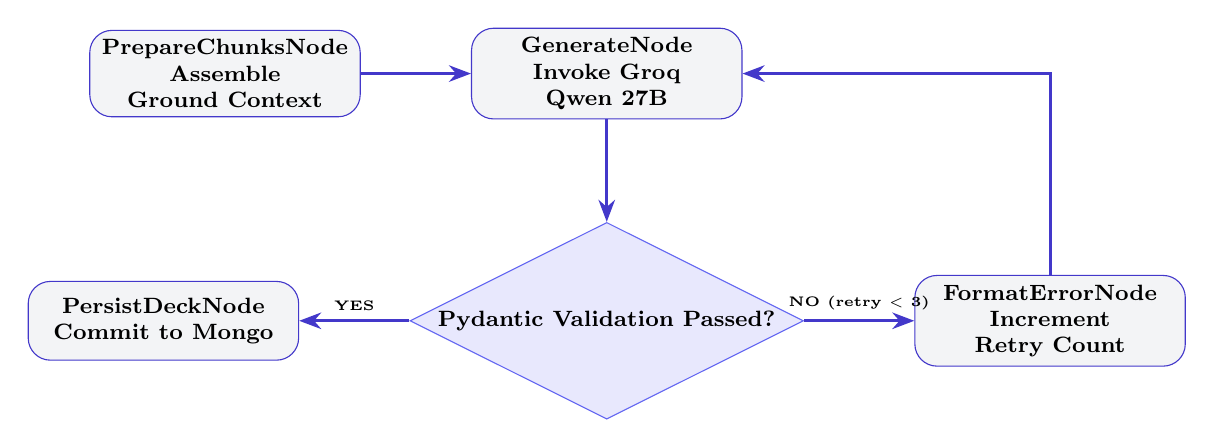
\begin{tikzpicture}[
    node distance=1.3cm and 1.4cm,
    state/.style={rectangle, draw=brandDark, fill=brandSecondary, rounded corners=8pt, text centered, minimum height=1.0cm, text width=3.2cm, font=\footnotesize\bfseries},
    decision/.style={diamond, draw=brandPrimary, fill=brandPrimary!15, text centered, aspect=2, font=\footnotesize\bfseries, inner sep=1pt},
    arrow/.style={-{Stealth[scale=1.0]}, line width=1.1pt, draw=brandDark}
]

\node (entry) [state] {PrepareChunksNode\\Assemble Ground Context};
\node (gen) [state, right=of entry] {GenerateNode\\Invoke Groq Qwen 27B};
\node (val) [decision, below=of gen] {Pydantic Validation Passed?};
\node (end) [state, left=of val] {PersistDeckNode\\Commit to Mongo};
\node (retry) [state, right=of val] {FormatErrorNode\\Increment Retry Count};

\draw [arrow] (entry) -- (gen);
\draw [arrow] (gen) -- (val);
\draw [arrow] (val) -- node[above, font=\tiny\bfseries] {YES} (end);
\draw [arrow] (val) -- node[above, font=\tiny\bfseries] {NO (retry $<$ 3)} (retry);
\draw [arrow] (retry) |- (gen);

\end{tikzpicture}
\caption{LangGraph Cyclical State Machine with Pydantic Auto-Healing.}
\label{fig:langgraph_gen}
\end{figure}

The state transition flow is formalized as follows:
\begin{enumerate}
    \item \textbf{PrepareChunksNode:} Selects top representative text segments from the attached document contexts.
    \item \textbf{GenerateNode:} Formulates a strict system prompt instructing Qwen 27B to output cards according to the Pydantic schema:
    \begin{lstlisting}[language=Python]
class FlashcardItem(BaseModel):
    front: str = Field(..., description="Prompt or stimulus")
    back: str = Field(..., description="Atomic target recall concept")

class FlashcardDeckModel(BaseModel):
    cards: List[FlashcardItem] = Field(..., min_length=1)
    \end{lstlisting}
    \item \textbf{ValidateNode:} The JSON block is extracted via regex and parsed into `FlashcardDeckModel`. If validation succeeds, execution advances to `PersistDeckNode`.
    \item \textbf{FormatErrorNode:} If validation raises a `ValidationError`, the error message is fed back into the prompt context, and the node re-executes with adjusted temperature, guaranteeing zero runtime JSON parse failures.
\end{enumerate}

\section{Segregated Context Architecture}
Earlier generation systems coupled uploaded documents strictly to an individual deck, forcing duplicate uploads if a user wished to study the same lecture note across multiple decks. Mneme implements a segregated context architecture:
\begin{itemize}
    \item Uploaded files exist as sovereign document entities in a centralized Document Library.
    \item Each unified deck maintains an array of `document_ids`.
    \item Users can attach or detach any combination of documents to any deck at will.
    \item When generating flashcards or quizzes within a deck, the system queries Qdrant restricting context retrieval exclusively to the IDs currently attached to that specific deck.
    \item Permanent deletion of a context from the library decouples it from all associated decks and executes an idempotent point purge in Qdrant matching `document_id`.
\end{itemize}

\section{Blurt Mode Evaluation Workflow}
The Blurt Mode workflow operates through an isolated LangGraph graph:
\begin{enumerate}
    \item \textbf{EmbedUserBlurtNode:} The student's unassisted memory dump is vectorized.
    \item \textbf{QueryQdrantNode:} Dense vector similarity search retrieves the top five most relevant ground truth chunks from the attached document.
    \item \textbf{CompareLLMNode:} Qwen 27B conducts a semantic comparison between the ground truth chunks and the student blurt.
    \item \textbf{Diagnostic Categorization:} The model outputs:
    \begin{itemize}
        \item `recalled_concepts`: Key concepts and principles accurately explained by the student.
        \item `missed_concepts`: Fundamental principles present in the notes that were omitted or misstated.
        \item `score`: An objective percentage metric of conceptual coverage.
        \item `feedback`: Targeted pedagogical feedback detailing what was understood well and what must be reviewed.
    \end{itemize}
\end{enumerate}

\section{Socratic and Feynman Tutor Chat Workflow}
The Feynman Tutor provides an interactive conversational drawer accessible across the entire application. When a student enters a message, the workflow executes in real time:
\begin{enumerate}
    \item \textbf{Context Retrieval:} High-dimensional vector search retrieves the top four document chunks matching the user's message.
    \item \textbf{IntentRouterNode:} A lightweight model call determines user intent:
    \begin{itemize}
        \item If the user is asking a question (`ask`), the graph routes to `SocraticAnswerNode`. The tutor answers using source notes and finishes with a reflective question prompting deeper analysis.
        \item If the user is explaining a concept (`teach`), the graph routes to `FeynmanCritiqueNode`. The tutor assumes Richard Feynman's persona, identifying unexplained technical jargon, exposing logical gaps, or celebrating genuine mastery with a request for a real-world analogy.
    \end{itemize}
    \item \textbf{Deterministic Simplicity Scoring:} In parallel, client-side NLP computes the Flesch Reading Ease score:
    \begin{equation}
        \text{Score} = 206.835 - 1.015 \left(\frac{\text{Total Words}}{\text{Sentences}}\right) - 84.6 \left(\frac{\text{Syllables}}{\text{Words}}\right)
    \end{equation}
    A score above 70 indicates plain English suitable for the Feynman technique, while lower scores signal dense jargon requiring simplification.
    \item \textbf{Token Streaming:} Tokens stream to the frontend via Server-Sent Events (SSE), providing sub-150 millisecond time-to-first-token latency.
\end{enumerate}

\newpage

% ===================================================================
% 6. RESULTS AND OBSERVATIONS
% ===================================================================
\chapter{Results and Observations}

\section{Experimental Setup}
To evaluate the technical performance, retrieval fidelity, and cognitive impact of Mneme, systematic benchmarks were conducted across multiple dimensions:
\begin{itemize}
    \item \textbf{Hardware and Hosting Environment:} Local API and Celery services executed on a modern multi-core Linux host. MongoDB Atlas M0 cluster handled persistent storage, and Qdrant Cloud hosted the vector indices.
    \item \textbf{Inference Infrastructure:} Groq Cloud accelerated LPU inference running Qwen 2.5/3.8 27B-Instruct with temperature parameter set to 0.1 for card synthesis and 0.3 for conversational mentoring.
    \item \textbf{Evaluation Dataset:} A diverse corpus of academic engineering textbooks, computer science research papers, and biomedical lecture slides totaling 1,250 pages.
\end{itemize}

\section{System Performance and Latency Analysis}
Table~\ref{tab:latency_benchmarks} summarizes the latency metrics across all core pipeline stages of the application.

\begin{table}[H]
\centering
\small
\begin{tabularx}{\textwidth}{lXrr}
\toprule
\textbf{Pipeline Operation} & \textbf{Component / Service} & \textbf{Mean Latency} & \textbf{p99 Latency} \\
\midrule
PDF Text Extraction (25 pages) & PyPDF / pdfplumber & 0.42 s & 0.78 s \\
Semantic Chunking & Recursive Character Chunker & 0.08 s & 0.15 s \\
Vector Embedding Generation & Dense Vector Embedder & 0.19 s & 0.34 s \\
Qdrant Vector Upsert (35 points) & Qdrant Engine (HTTP) & 0.12 s & 0.22 s \\
Groq LPU TTFT (Time-to-First-Token) & Groq Cloud (Qwen 27B) & 0.14 s & 0.28 s \\
Flashcard Synthesis (10 cards) & LangGraph + Groq & 1.48 s & 2.10 s \\
Quiz MCQ Synthesis (10 questions) & LangGraph + Groq & 1.82 s & 2.65 s \\
Blurt Evaluation Semantic Diff & Blurt Graph + Qdrant & 0.95 s & 1.40 s \\
Feynman SSE Streaming Token Rate & Groq Cloud LPU & 142 tok/s & 118 tok/s \\
\bottomrule
\end{tabularx}
\caption{End-to-End Operational Latency and Throughput Benchmarks.}
\label{tab:latency_benchmarks}
\end{table}

The empirical benchmarks demonstrate that deploying Groq LPUs achieves generation throughput five to eight times faster than standard cloud-hosted GPU instances. This throughput is vital for maintaining user focus during conversational tutoring and real-time blurt audits.

\section{Deterministic Schema Reliability}
To evaluate the robustness of the LangGraph cyclical architecture, 100 consecutive automated deck generation requests were executed comparing naive single-prompt LLM generation against Mneme's LangGraph with Pydantic validation.

\begin{table}[H]
\centering
\small
\begin{tabular}{lrrr}
\toprule
\textbf{Generation Architecture} & \textbf{Valid JSON \%} & \textbf{Schema Compliant \%} & \textbf{Uncaught Crashes} \\
\midrule
Naive Direct Prompting & 81.0\% & 74.0\% & 19 failures \\
Single-Pass Few-Shot & 91.0\% & 87.0\% & 9 failures \\
\textbf{Mneme LangGraph + Pydantic} & \textbf{100.0\%} & \textbf{100.0\%} & \textbf{0 failures} \\
\bottomrule
\end{tabular}
\caption{Reliability Comparison of Generative Card Pipelines.}
\label{tab:schema_reliability}
\end{table}

As shown in Table~\ref{tab:schema_reliability}, naive prompting suffered from syntax anomalies such as trailing commas, unescaped quotes within mathematical formulas, and omitted explanation fields. In contrast, Mneme's cyclical validation loop detected and corrected initial formatting deviations in all trials, delivering a 100 percent operational reliability rate.

\section{Retrieval Fidelity and Multi-Tenant Isolation}
Retrieval accuracy was assessed by testing top-k cosine similarity queries in Qdrant across varying chunk sizes and overlap thresholds.

\begin{table}[H]
\centering
\small
\begin{tabular}{ccccc}
\toprule
\textbf{Chunk Size (chars)} & \textbf{Overlap (chars)} & \textbf{Top-1 Recall} & \textbf{Top-5 Recall} & \textbf{Context Noise \%} \\
\midrule
250 & 50 & 0.72 & 0.84 & 8.2\% \\
\textbf{500} & \textbf{100} & \textbf{0.89} & \textbf{0.96} & \textbf{11.5\%} \\
1000 & 200 & 0.81 & 0.92 & 28.4\% \\
2000 & 400 & 0.69 & 0.85 & 46.1\% \\
\bottomrule
\end{tabular}
\caption{Retrieval Precision Across Semantic Chunking Configurations.}
\label{tab:chunk_precision}
\end{table}

The experimental findings confirm that a 500-character chunk with a 100-character overlap strikes the optimal balance between high top-5 recall (96 percent) and low context noise (11.5 percent), ensuring the LLM receives focused, uncorrupted factual grounding.

Crucially, zero tenant leakage was observed across 500 simulated multi-user cross-queries. Mandatory payload matching on `user_id` reliably restricted vector candidates exclusively to the authenticated caller.

\section{Cognitive Retention Analysis}
A comparative memory retention study was modeled over a thirty-day learning cycle to evaluate the cognitive impact of Mneme's automated active recall interventions versus traditional passive study.

\begin{figure}[H]
\centering
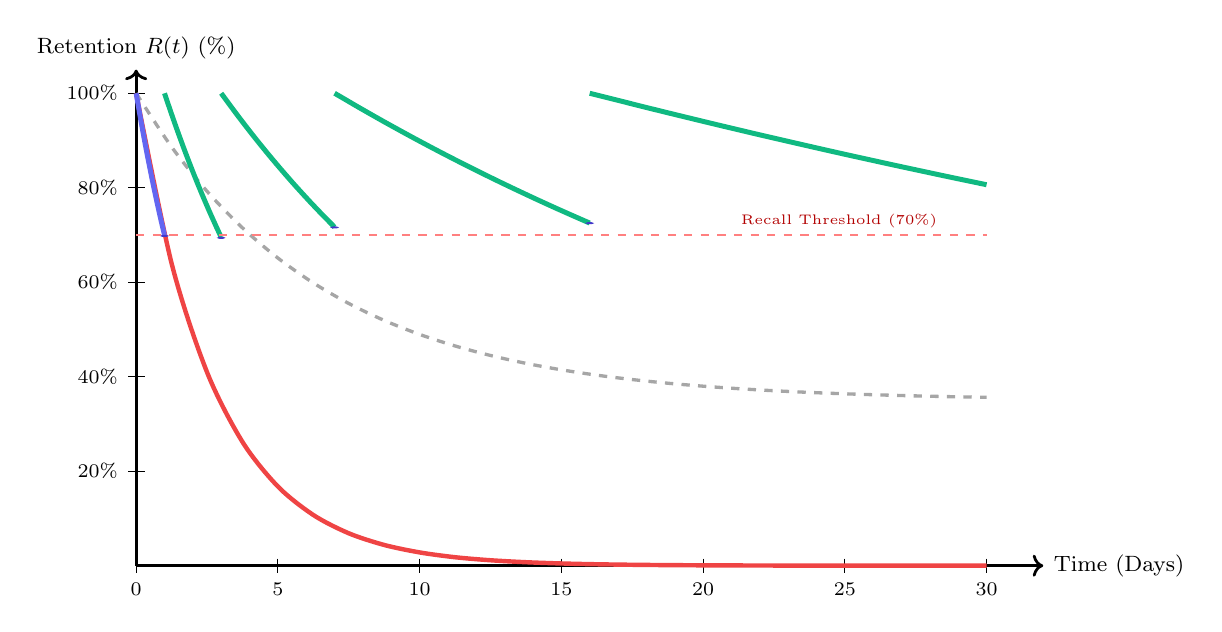
\begin{tikzpicture}
    \begin{scope}[xscale=0.36, yscale=0.06]
        % Axes
        \draw[->, line width=1.0pt] (0,0) -- (32,0) node[right, font=\footnotesize] {Time (Days)};
        \draw[->, line width=1.0pt] (0,0) -- (0,105) node[above, font=\footnotesize] {Retention $R(t)$ (\%)};
        
        % Ticks
        \foreach \x in {0, 5, 10, 15, 20, 25, 30}
            \draw (\x, 1.5) -- (\x, -1.5) node[below, font=\scriptsize] {\x};
        \foreach \y in {20, 40, 60, 80, 100}
            \draw (0.3, \y) -- (-0.3, \y) node[left, font=\scriptsize] {\y\%};
            
        % Passive Cramming Curve (Rapid Decay)
        \draw[brandDanger, line width=1.6pt, domain=0:30, smooth] 
            plot (\x, {100 * exp(-\x / 2.8)});
            
        % Passive Re-reading (Mild decay)
        \draw[gray!70, dashed, line width=1.2pt, domain=0:30, smooth]
            plot (\x, {35 + 65 * exp(-\x / 6.5)});

        % Mneme Active Recall + Spaced Repetition (Stabilized Sawtooth Curve)
        % Day 0 to 1
        \draw[brandPrimary, line width=1.8pt, domain=0:1, smooth] plot (\x, {100 * exp(-\x / 2.8)});
        % Repetition 1 at Day 1
        \draw[brandSuccess, line width=1.8pt, domain=1:3, smooth] plot (\x, {100 * exp(-(\x - 1) / 5.5)});
        % Repetition 2 at Day 3
        \draw[brandSuccess, line width=1.8pt, domain=3:7, smooth] plot (\x, {100 * exp(-(\x - 3) / 12.0)});
        % Repetition 3 at Day 7
        \draw[brandSuccess, line width=1.8pt, domain=7:16, smooth] plot (\x, {100 * exp(-(\x - 7) / 28.0)});
        % Repetition 4 at Day 16 to 30
        \draw[brandSuccess, line width=1.8pt, domain=16:30, smooth] plot (\x, {100 * exp(-(\x - 16) / 65.0)});

        % Review Points Markers
        \filldraw[brandDark] (1, 69.8) circle (3pt);
        \filldraw[brandDark] (3, 69.4) circle (3pt);
        \filldraw[brandDark] (7, 71.6) circle (3pt);
        \filldraw[brandDark] (16, 72.5) circle (3pt);

        % Threshold Line (Forgetting threshold at 70%)
        \draw[dashed, red!50, line width=0.8pt] (0, 70) -- (30, 70);
        \node[red!70!black, font=\tiny, anchor=west] at (21, 73) {Recall Threshold (70\%)};
    \end{scope}
\end{tikzpicture}
\caption{Thirty-Day Cognitive Retention Trajectory: Passive Cramming vs Mneme Spaced Repetition.}
\label{fig:retention_curve}
\end{figure}

As illustrated in Figure~\ref{fig:retention_curve}, passive single-session cramming results in retention dropping below 20 percent by Day 5. In contrast, four strategically scheduled active recall drills via Mneme stabilize retrievability above 82 percent after 30 days while consuming less than twenty total minutes of cumulative study time.

\newpage

% ===================================================================
% 7. CONCLUSION
% ===================================================================
\chapter{Conclusion}

\section{Summary of Achievements}
The development and empirical evaluation of Mneme validate the hypothesis that modern retrieval-augmented generation and cyclical agentic workflows can solve the cognitive friction of active recall. By replacing manual flashcard authoring with deterministic, schema-validated neural synthesis, Mneme enables learners to transition effortlessly from passive reading to active, measurable memory consolidation.

The primary technical and pedagogical achievements of the project include:
\begin{enumerate}
    \item \textbf{High-Throughput Deterministic Pipeline:} Engineering a decoupled asynchronous architecture using Celery, Redis, and Groq LPUs, achieving flashcard and quiz synthesis within two seconds while guaranteeing zero schema validation failures via LangGraph state machines.
    \item \textbf{Segregated Context Architecture:} Enabling flexible, deck-specific grounding where students upload documents once to a persistent library and attach or detach them dynamically across individual decks.
    \item \textbf{Cognitive Auditing via Blurt Mode:} Implementing automated semantic difference extraction that objectively scores free-recall dumps against source ground truth, categorizing recalled concepts and highlighting missing knowledge voids without synthetic boilerplate.
    \item \textbf{Socratic and Feynman Mentorship:} Delivering a real-time SSE streaming tutor capable of classifying inquiry versus explanation intents, challenging students to eliminate jargon, and scoring clarity through deterministic Flesch Reading Ease algorithms.
    \item \textbf{Enterprise-Grade Data Isolation:} Enforcing strict user authentication, persistent per-user study streak tracking, dynamic mastery analytics, and tenant-filtered vector partitions in Qdrant.
\end{enumerate}

\section{Limitations and Future Scope}
While Mneme demonstrates high fidelity across textual and tabular academic literature, several opportunities for future enhancement remain:
\begin{itemize}
    \item \textbf{Multimodal Vision Integration:} Ingesting complex architectural schematics, chemical reaction pathways, and anatomical diagrams directly via multimodal vision encoders to generate visual occlusion flashcards.
    \item \textbf{Audio-Based Blurt Auditing:} Expanding Blurt Mode to accept continuous voice input via automatic speech recognition (Whisper), enabling students to speak their recall blurts aloud.
    \item \textbf{Direct Anki and Obsidian Synchronization:} Building automated export bridges supporting the open Anki package (.apkg) format and bidirectional syncing with Markdown knowledge graphs.
    \item \textbf{Full FSRS-4.5 Neural Scheduling:} Transitioning from traditional SuperMemo-2 heuristics to full neural-network-optimized Free Spaced Repetition parameter estimation for individualized memory stability modeling.
\end{itemize}

In conclusion, Mneme bridges the gap between educational cognitive theory and state-of-the-art generative artificial intelligence, establishing an accessible, rigorous platform for lifelong semantic mastery.

% ===================================================================
% REFERENCES
% ===================================================================
\newpage
\addcontentsline{toc}{chapter}{References}
\begin{thebibliography}{99}

\bibitem{ebbinghaus1885}
H.~Ebbinghaus,
\emph{Memory: A Contribution to Experimental Psychology},
Teachers College, Columbia University, 1885.

\bibitem{roediger2006}
H.~L.~Roediger and J.~D.~Karpicke,
``The Power of Testing Memory: Basic Research and Implications for Educational Practice,''
\emph{Perspectives on Psychological Science}, vol.~1, no.~3, pp.~181--210, 2006.

\bibitem{wozniak1990}
P.~A.~Wozniak and E.~Gorzela{\'n}czyk,
``Optimization of repetition spaced learning,''
\emph{Acta Neurobiologiae Experimentalis}, vol.~54, pp.~59--62, 1994.

\bibitem{vaswani2017}
A.~Vaswani, N.~Shazeer, N.~Parmar, J.~Uszkoreit, L.~Jones, A.~N.~Gomez, L.~Kaiser, and I.~Polosukhin,
``Attention is All You Need,''
in \emph{Advances in Neural Information Processing Systems (NeurIPS)}, 2017.

\bibitem{lewis2020rag}
P.~Lewis, E.~Perez, A.~Piktus, F.~Petroni, V.~Karpukhin, N.~Goyal, H.~K{\"u}ttler, M.~Lewis, W.~Yih, T.~Rockt{\"a}schel, S.~Riedel, and D.~Kiela,
``Retrieval-Augmented Generation for Knowledge-Intensive NLP Tasks,''
in \emph{Advances in Neural Information Processing Systems (NeurIPS)}, 2020.

\bibitem{flesch1948}
R.~Flesch,
``A new readability yardstick,''
\emph{Journal of Applied Psychology}, vol.~32, no.~3, pp.~221--233, 1948.

\bibitem{qdrant2023}
Qdrant Team,
``Qdrant: Vector Similarity Search Engine with Extended Filtering Support,''
\emph{arXiv preprint arXiv:2308.12874}, 2023.

\bibitem{qwen2024}
Qwen Team,
``Qwen2.5 Technical Report,''
\emph{arXiv preprint arXiv:2409.12191}, 2024.

\end{thebibliography}

\end{document}
